\documentclass[]{article}

\usepackage{amsmath}  % AMS math package
\usepackage{amssymb}  % AMS symbol package
\usepackage{bm}       % bold math
\usepackage{graphicx} % Include figure files
\usepackage{dcolumn}  % Align table columns on decimal point
\usepackage{multirow} % Multirow/column tables
\usepackage{hyperref} % Hyperlinks
\usepackage{caption}
\usepackage{subcaption}

\begin{document}

\title{Ising Model}
\author{Justin Browne}
\date{}
\maketitle

\begin{abstract}
This work covers the development and application of a monte carlo program to simulate the Ising Model. The monte carlo method used is the Metropolis algorithm. The program is used to study how a lattice of spins reacts to different external fields, initial lattice configurations, temperatures, and boundary conditons.
\end{abstract}

\section{Introduction}
The Ising Model is a model used to describe magnetism in a lattice in which each lattice site can have a spin $\sigma_{i} = \pm 1$.
The interaction is described by the Hamiltonian
\[
H = - \sum_{<i~j>} J_{ij} \sigma_i \sigma_j -\mu \sum_{i} h_i \sigma_i ~,
\]
where $J_{ij}$ is the interaction between lattice sites $i$ and $j$, $\mu$ is the magnetic moment, $h_{i}$ is the magnetic field at lattice site $i$, and $\sum_{i~j}$ indicates a sum among only nearest neighbors.

This model is a very important model in statistical mechanics. It is a simple model, and was the first with a phase transition to be solved exactly \cite{mccoy2012}.

\section{Implementation}
The implementation of the Ising model in this work has incorporated a few simplifications.
First, the field is assumed to be equal everywhere ($h_{i} = h$).
Second, the interaction between spins are assumed to be the same ($J_{ij} = J$). This means the Hamiltonian is
\[
H = - J \sum_{<i~j>} \sigma_i \sigma_j -\mu h \sum_{i} \sigma_i ~.
\]

The system is simulated using the Metropolis algorithm\cite{metropolis1953} as follows:
\begin{enumerate}
	\item Choose an initial lattice configuration.
	\item Choose a random point, $P$, on the lattice.
	\item If flipping the spin at $P$ is energetically favorable, flip the spin.
		If it is not, flip the spin with a probability of $e^{-\beta \Delta \! H}$, where $\Delta \! H$ is the difference between the Hamiltonian before and after the proposed spin flip.
		\[
			\sigma_{P,n+1} =
			\begin{cases}
				-\sigma_{P,n} & \text{if } \Delta \! H < 0 \\
				-\sigma_{P,n} & \text{if } \Delta \! H > 0 \wedge r < e^{- \beta \Delta \! H} \\
				\phantom{-}\sigma_{P,n} & \text{otherwise}
			\end{cases}
		\]
		where $\beta = \frac{1}{k_{B} T}$ is the inverse temperature, and $r$ is a random number from a uniform distriution spanning $[0,1)$.
	\item Repeat from step 2.
\end{enumerate}

All simulations in this work are performed using a $50 \times 50$ grid, with $J=1$, unless otherwise specified.

\section{System Convergence}
The system converged at rates that varied depending on many variables, such as the initial configuration, the external field, and the temperature.

The temperature affects the rate of convergence because the temperature determines the probability of a spin flip, which would not be energetically favorable, occuring. This means the system is more likely to escape from a local minimum. Figure~\ref{fig:conv_beta} shows how convergence varies with $\beta$.

\begin{figure}[htb]
	\centering
	\begin{subfigure}[b]{.9\textwidth}
		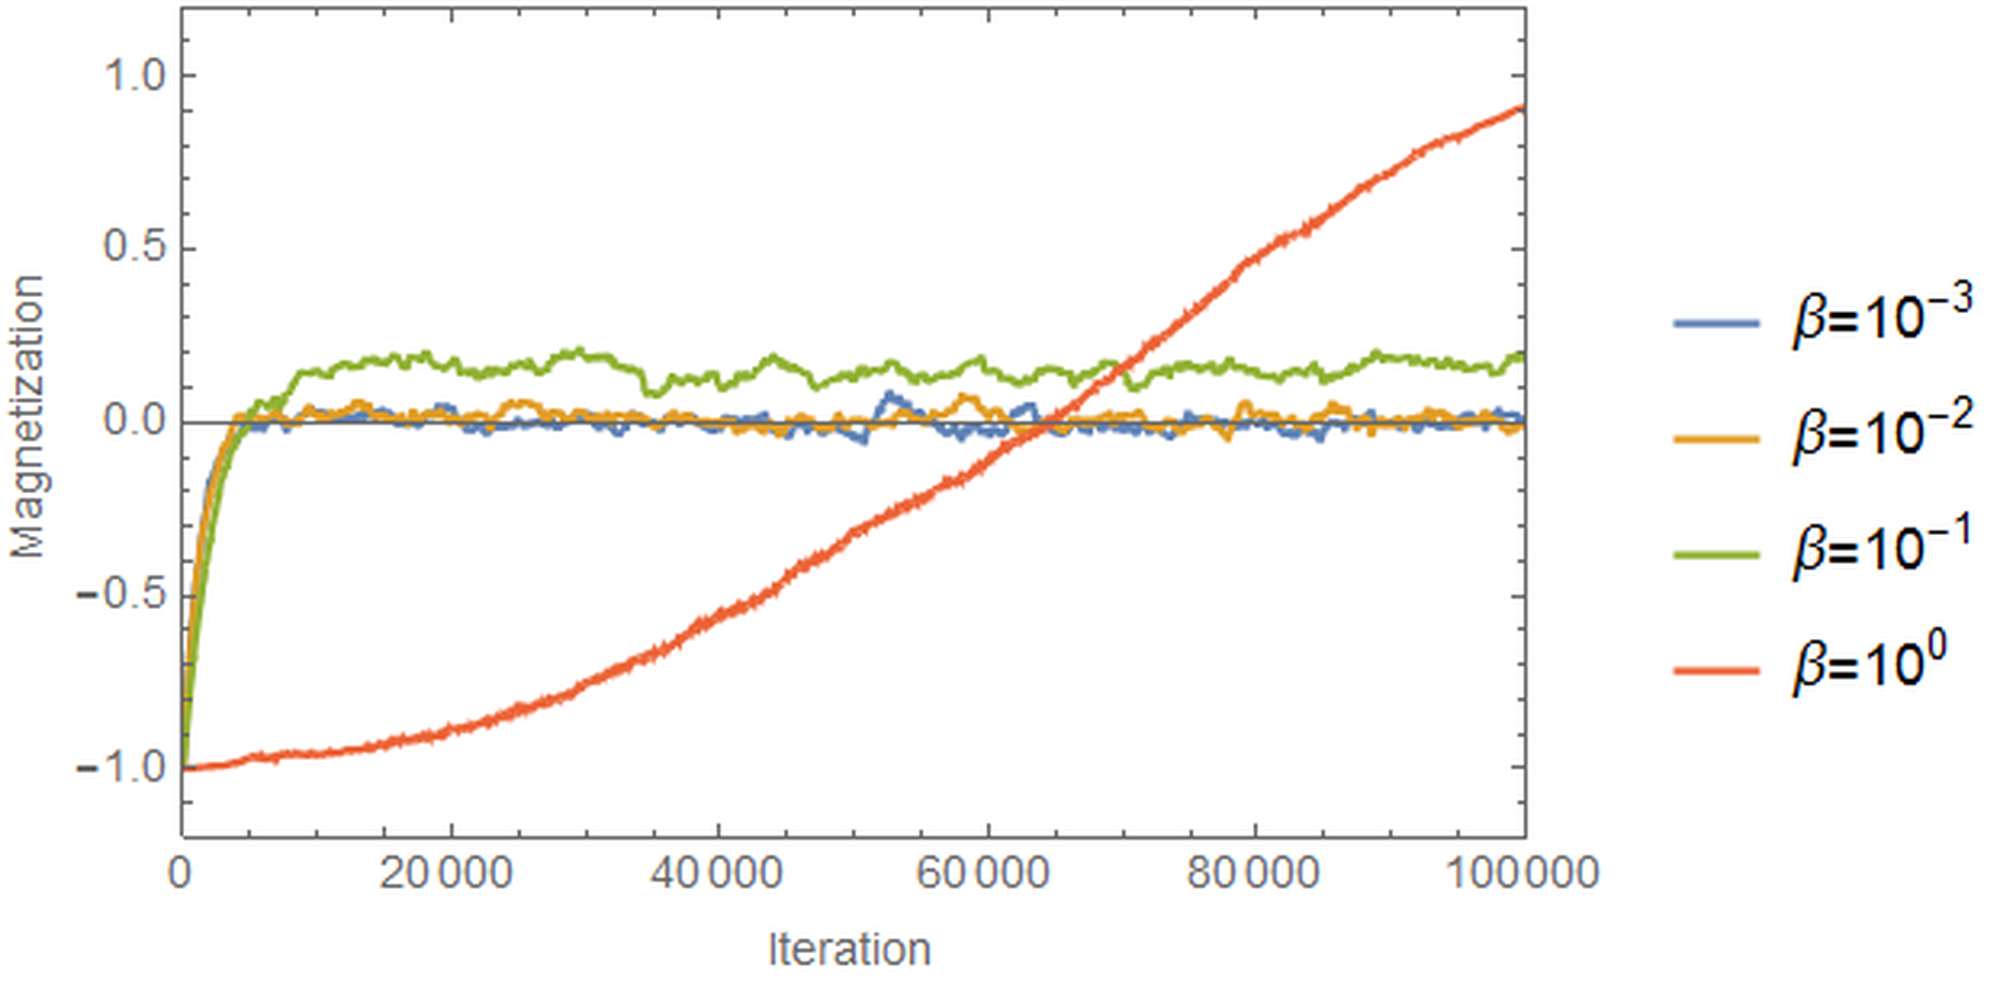
\includegraphics[width=\textwidth]{figures/m_v_t_beta_out.png}
	\end{subfigure}\\
	\begin{subfigure}[b]{.9\textwidth}
		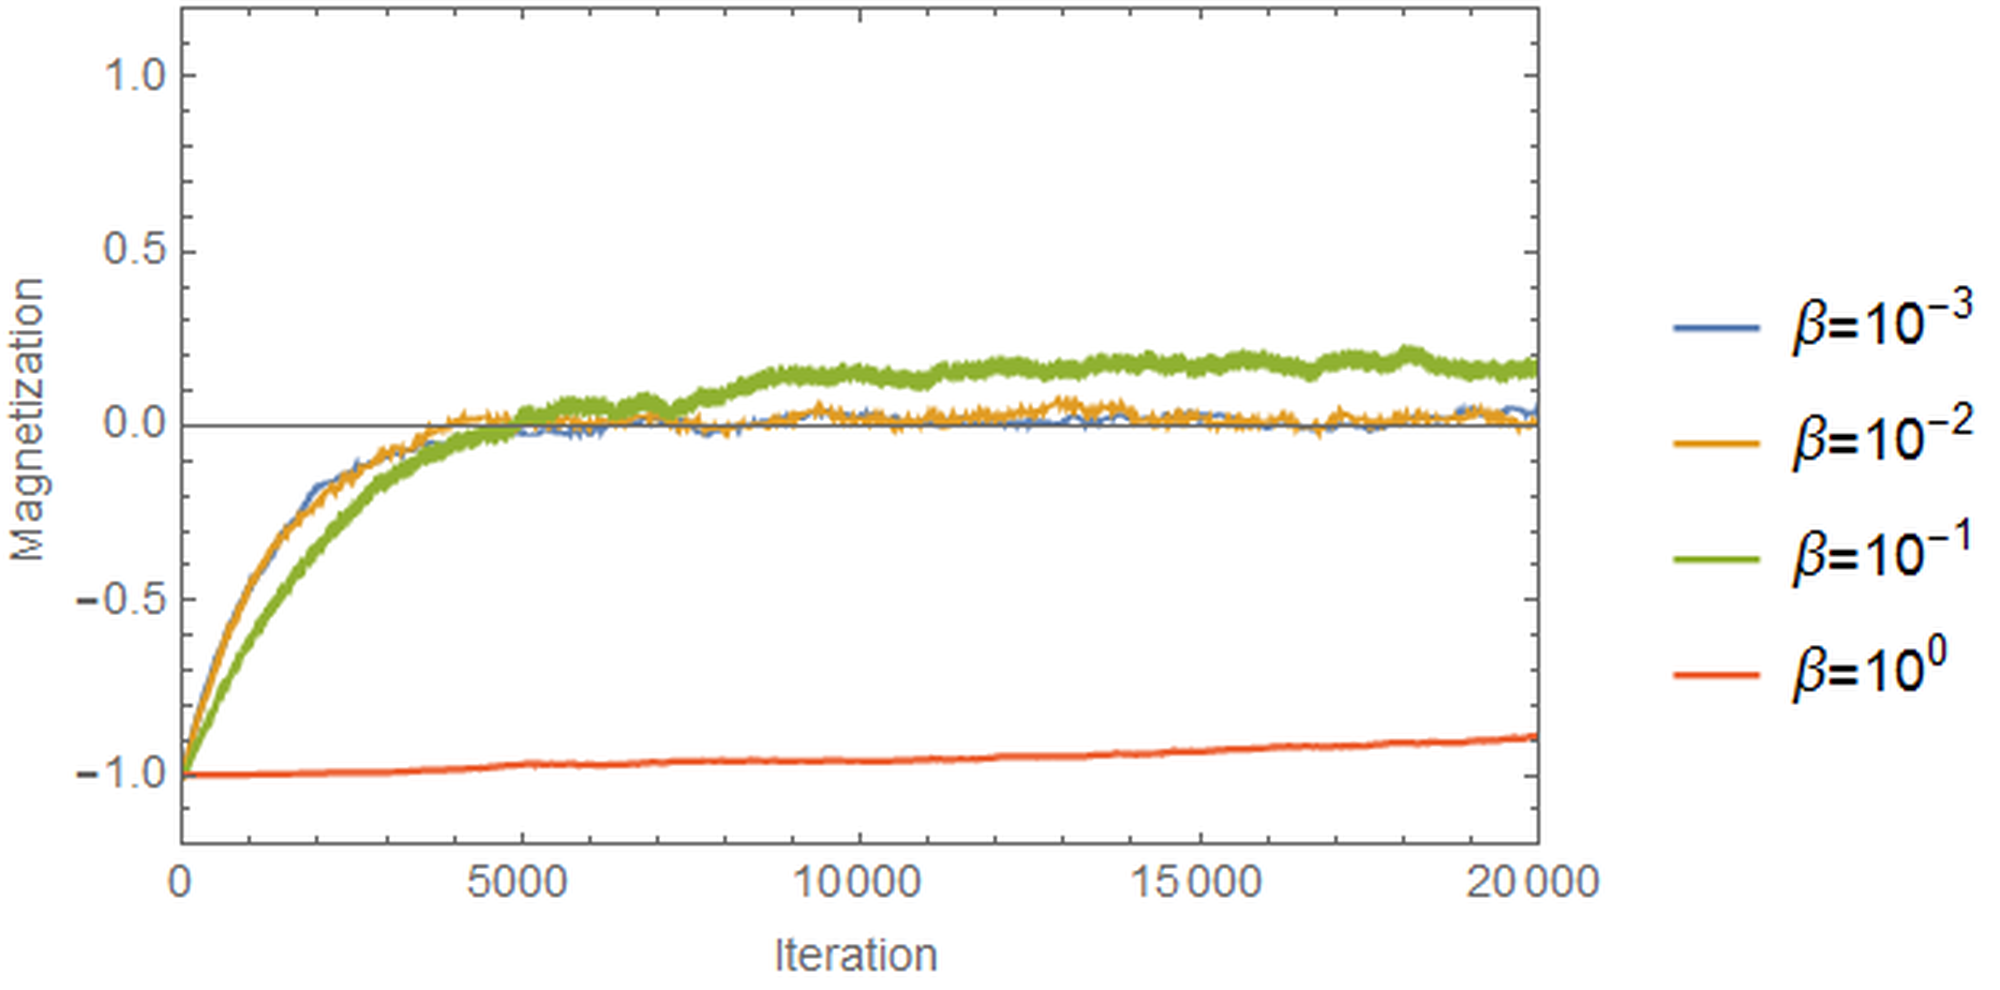
\includegraphics[width=\textwidth]{figures/m_v_t_beta_in.png}
	\end{subfigure}
	\caption{The magnetization versus iteration number for various temperatures, zoomed out (top) and in (bottom). The higher temperature (lower $\beta$) runs converge faster. For these simulaltions, the field interaction was $\mu h = +1$, and all of the spins were initially aligned down.}
	\label{fig:conv_beta}
\end{figure}

Whether the boundaries are periodic or not affects the convergence as well.
Since the sites on the edge of the lattice interact with fewer sites, their spins are more likely to flip.
This means they act as nucleation sites.
Figure~\ref{fig:nucleation} shows the lattice of a non-periodic lattice at various points through the simulation, and figure~\ref{fig:conv_per} shows how the convergence depends on the boundary conditions.

\begin{figure}[htb]
	\centering
	\begin{subfigure}[b]{.3\textwidth}
		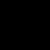
\includegraphics[width=\textwidth]{figures/lattice1_1.png}
	\end{subfigure}
	\begin{subfigure}[b]{.3\textwidth}
		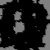
\includegraphics[width=\textwidth]{figures/lattice1_2.png}
	\end{subfigure}
	\begin{subfigure}[b]{.3\textwidth}
		
\includegraphics[width=\textwidth]{figures/lattice1_3.png}
	\end{subfigure}
	\caption{The lattice of a simulation with $\beta = 1$, $\mu h = +1$, at the beginning of (left), midway through (center), and at the end of (right) of the simulation. The lattice boundaries are non-periodic. Spin flips tend to propagate from the edges toward the center.}
	\label{fig:nucleation}
\end{figure}

\begin{figure}[htb]
	\centering
	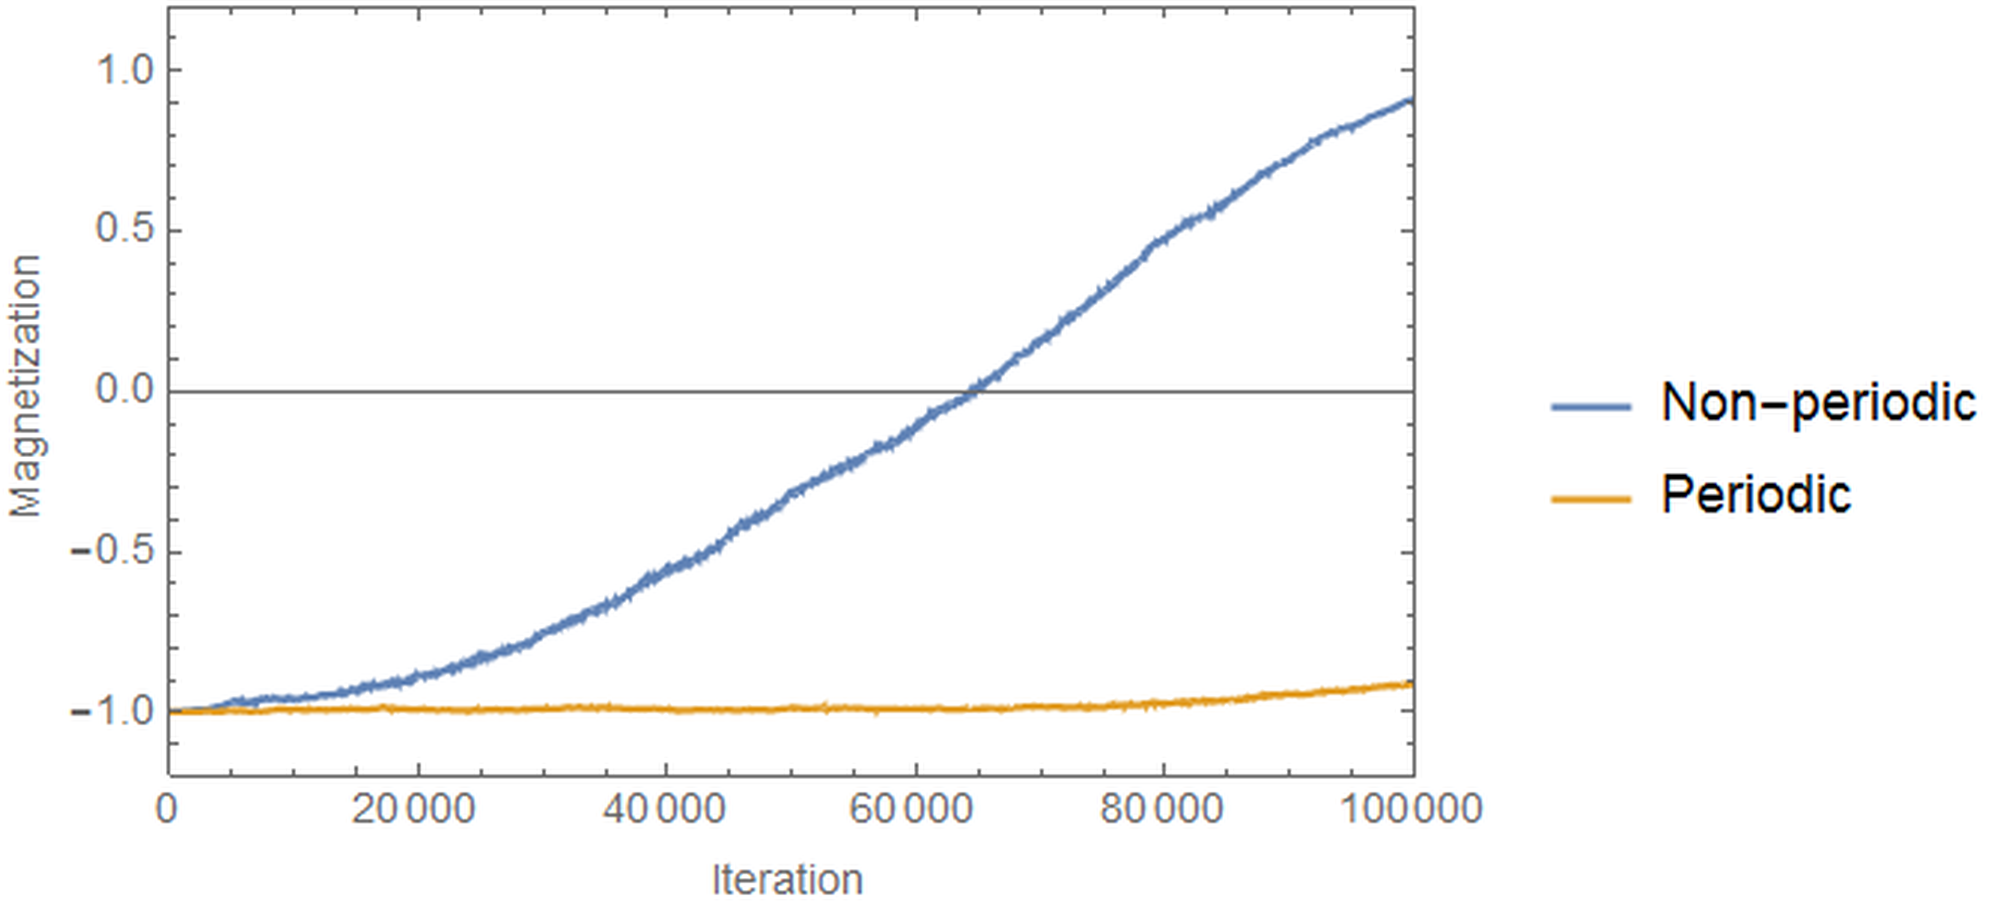
\includegraphics[width=\textwidth]{figures/m_v_t_per.png}
	\caption{The magnetization versus iteration number for periodic and non-periodic boundaries. The simulation with non-periodic boundaries more quickly escaped the local minimum.}
	\label{fig:conv_per}
\end{figure}

\section{Temperature Dependence}
Varying the temperature of the system shows some interesting properties.
At low temperatures, the system prefers a configuration in which all the spins are aligned.
At high temperatures, the system tends to prefer a randomized configuration.
The temperature around which the system undergoes this change is called the Curie Temperature.
The system behavior around the Curie Temperature has been solved analytically \cite{osanger1944,montroll1963}.
The solution is of the form
\[
	M = (1-\sinh^{4}(2 \beta J))^{1/8} ~.
\]
This behavior can be seen in figure~\ref{fig:critical}.

\begin{figure}[htb]
	\centering
	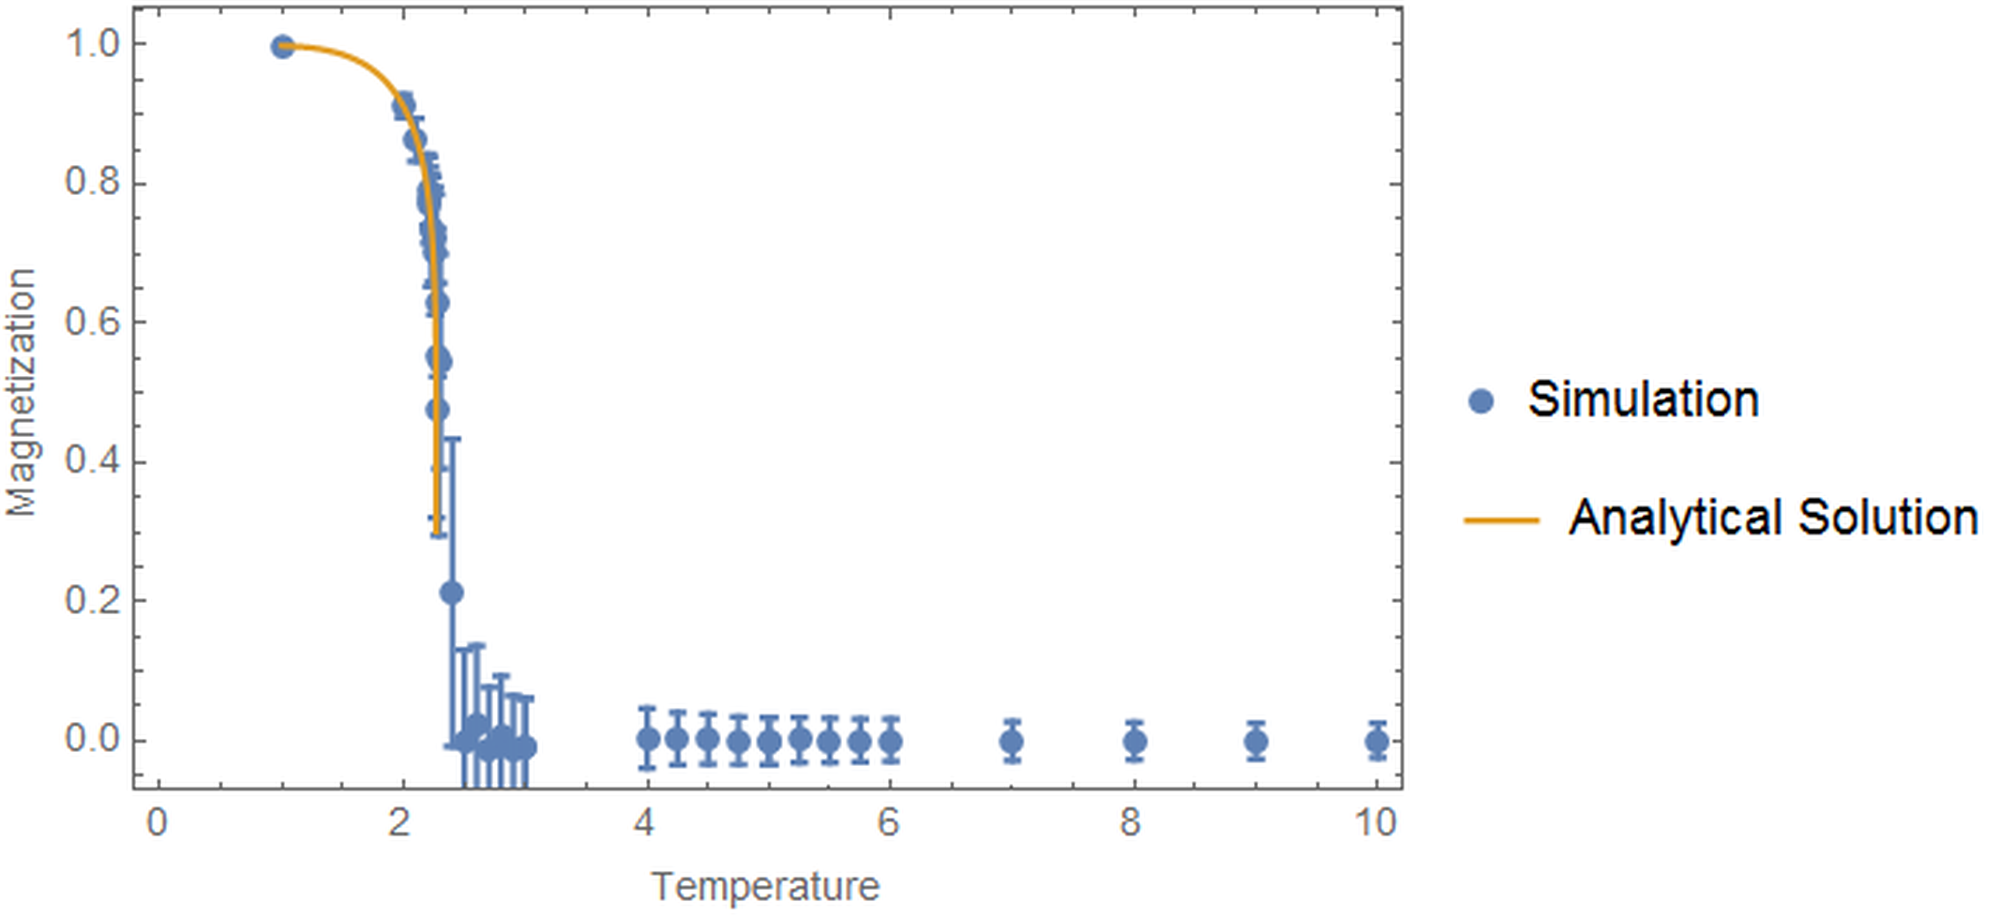
\includegraphics[width=\textwidth]{figures/m_v_T.png}
	\caption{The magnetization versus temperature. The simulation results and the analytical solution are show. For these simulations, $\mu h = 0$, the spins were initially aligned up, and the boundaries were periodic.}
	\label{fig:critical}
\end{figure}

Above the Curie temperature, all conditions result in a random configuration.
However, the system experiences bifurcation below the Curie Temperature.
Depending on the initial configuration and the external field, the system will settle to different stable configurations.
With an external field, the spins tend to align with the field.
However, without an external field, the spins tend to form domains of the same spin.
This means that low temperature systems with no external field that are initialized randomly act randomly and chaotically.
Different initial conditions and different random seeding greatly affect the outcome of the simulation.

\section{Further Study}
There are more aspects of the Ising model that could be explored.
This work only focused on systems with $J=1$, corresponds to ferromagnetic systems.
Studying antiferromagnetic systems could prove to be very interesting.
The scope of the program could be expanded to include non-uniform magnetic fields, non-uniform or long-range spin-spin interactions.

\begin{thebibliography}{}
	\bibitem{mccoy2012}
		McCoy, B.~M., \& Maillard, J.\ 2012, arXiv:1203.1456 
	\bibitem{metropolis1953}
		Metropolis, N., Rosenbluth, A.~W., Rosenbluth, M.~N., Teller, A.~H., \& Teller, E.\ 1953, Journal of Chemical Physics, 21, 1087 
	\bibitem{osanger1944}
		Onsager, Lars (1944), "Crystal statistics. I. A two-dimensional model with an order-disorder transition", Phys. Rev., Series II 65: 117–149
	\bibitem {montroll1963}
		Montroll, Elliott W. and Potts, Renfrey B. and Ward, John C., Journal of Mathematical Physics, 4, 308-322 (1963)
\end{thebibliography}

\end{document}
